\stepcounter{slidesection}
\setbeamertemplate{background}[bgfirst]
\setbeamertemplate{footline}[first]
\subtitle{\theslidesection: Next Generation Sequencing}
% TODO
\titlegraphic{Kapitel/TechnischeGrundlagen/Bilder/logo2.png}
\begin{frame}[noframenumbering]
    \titlepage
    \begin{textblock}{10}(4.75,15)
        \cite{ProgrammingLogo}
    \end{textblock}
\end{frame}
\setbeamertemplate{footline}[presentationbody] 
\setbeamertemplate{background}[bgbody]

\begin{frame}{Struktur}
	\begin{itemize}
		\item Klima(wandel) und Gesundheit
		\item Genomik und Next Generation Sequencing
		\item Ausatmen: ?
		\item NGS zur Untersuchung von Klimawandel
		\item Ausatmen: ?
		\item NGS zur Bewältigung von Klimawandel-Herausforderungen
	\end{itemize}
\end{frame}

\begin{frame}{Klima(wandel) und Gesundheit}
	\begin{itemize}
		\item Zusammenhang Klima und Gesundheit: Hippokrates
		\item Direkte Einflüsse:
		\begin{itemize}
			\item Temperatur (signifikanter Anstieg in den letzten 10 Jahren)
			\item Essensversorgung (Knappheit, Qualität)
			\item Wasserversorgung (WHO: 66$\%$ Wasserknappheit bis 2025)
			\item Verbreitung tropischer Krankheiten (Malaria, Rift Valley Fever, Dengue)
			\item Cholera: Überschwemmungen. ...Und Temperatur? 
		\end{itemize}
		\item Mentale Einflüsse:
		\begin{itemize}
			\item Depression bei Klimaforschern und -Journalisten - Pre-traumatic stress syndrome
			\item PTSD, erhöhte Selbstmordrate nach Klimakatastrophen (z.B. Katharina, Inuit)
			\item American Psychological Association: Natürliche Reaktionen wie Konfliktvermeidung, Resignation zunehmende Antwort auf Klimawandel (Effekt u.A.: Unfähigkeit zu reagieren)
			\item Zunehmende Anzahl an Schulabgängern, die nicht studieren wollen, da sie keine Zukunft sehen
			\item Zunehmende Abwägung: Kinderwunsch vs. Klimawandel (``Ich habe keine Kinder und einen Hund, und Gott sei dank wird der in 10 Jahren tot sein.''), Birth Strike
			\item Climate Health Professionals
			\item Aktivismus als Bewältigungsstrategie
		\end{itemize}
	\end{itemize}
\end{frame}

\begin{frame}{Interaktion}
	Welches prägnanteste oder interessanteste Beispiel für ein klimawandelbezogenes Ereignis, dessen Bezug zur Gesundheit Sie jetzt erkennen, fällt Ihnen aus der letzten Zeit ein? Unterhalten Sie sich kurz mit 1-2 benachbarten Studierenden. 
\end{frame}

\begin{frame}{Genomik und NGS}
\end{frame}

\begin{frame}{Interaktion}
	? 
\end{frame}

\begin{frame}{Untersuchung des Klimawandels}
	\begin{itemize}
		\item Phytoplankton-Sequenzierung in der Antarktis % https://www.earlham.ac.uk/articles/emma-langan-antarctic-adventure-algae-climate-change
		\item 
	\end{itemize}
\end{frame}

\begin{frame}{Geräte}
    \only<1->{
        \begin{textblock}{9.2}(1,3)
            \begin{mdframed}[backgroundcolor=white]
                \begin{center}
                    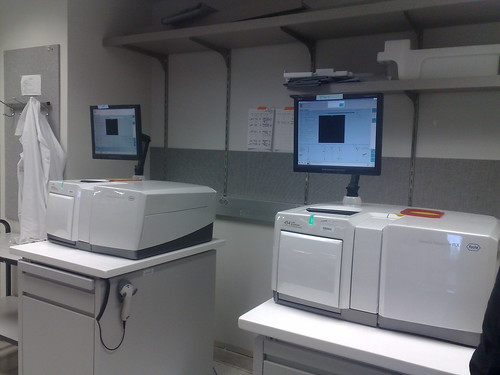
\includegraphics[height=5.2cm]{Kapitel/NGSTechnologien/Bilder/NGS454.jpg}\\
					\vspace{0.3cm}\captionof{figure}{Eins der ersten NGS-Geräte: Der Roche 454 (ca. 70k-700k Reads je 400-700 bp, bis ca. 500 Mbp)\cite{NGS454}}
                \end{center}
            \end{mdframed}
        \end{textblock}
    }
    \only<2->{
        \begin{textblock}{9.2}(2,3.1)
            \begin{mdframed}[backgroundcolor=white]
                \begin{center}
                    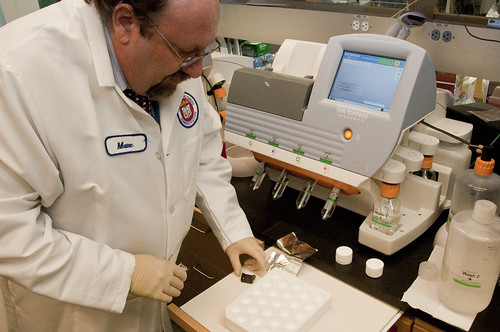
\includegraphics[height=5.2cm]{Kapitel/NGSTechnologien/Bilder/NGSPGM.jpg}\\
					\vspace{0.3cm}\captionof{figure}{Der spirituelle Nachfolger des 454: Der IonTorrent PGM (ca. 400k-4M Reads je 400 bp, bi ca. 1.6 Gbp)\cite{NGSPGM}}
                \end{center}
            \end{mdframed}
        \end{textblock}
    }
    \only<3->{
        \begin{textblock}{9.2}(3,3.2)
            \begin{mdframed}[backgroundcolor=white]
                \begin{center}
                    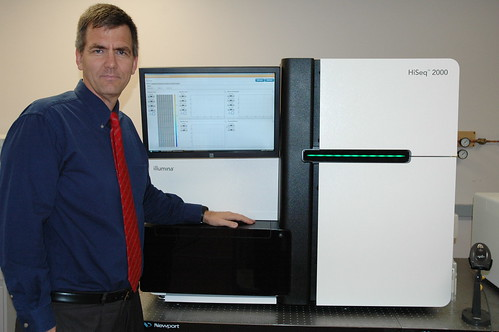
\includegraphics[height=5.2cm]{Kapitel/NGSTechnologien/Bilder/NGSHiSeq.jpg}\\
					\vspace{0.3cm}\captionof{figure}{Das Hauptgerät des aktuellen Marktführers: Ein Illumina HiSeq (ca. 2000M Reads je 250 bp, bis ca. 500 Gbp)\cite{NGSHiSeq}}
                \end{center}
            \end{mdframed}
        \end{textblock}
    }
    \only<4->{
        \begin{textblock}{9.2}(4,3.3)
            \begin{mdframed}[backgroundcolor=white]
                \begin{center}
                    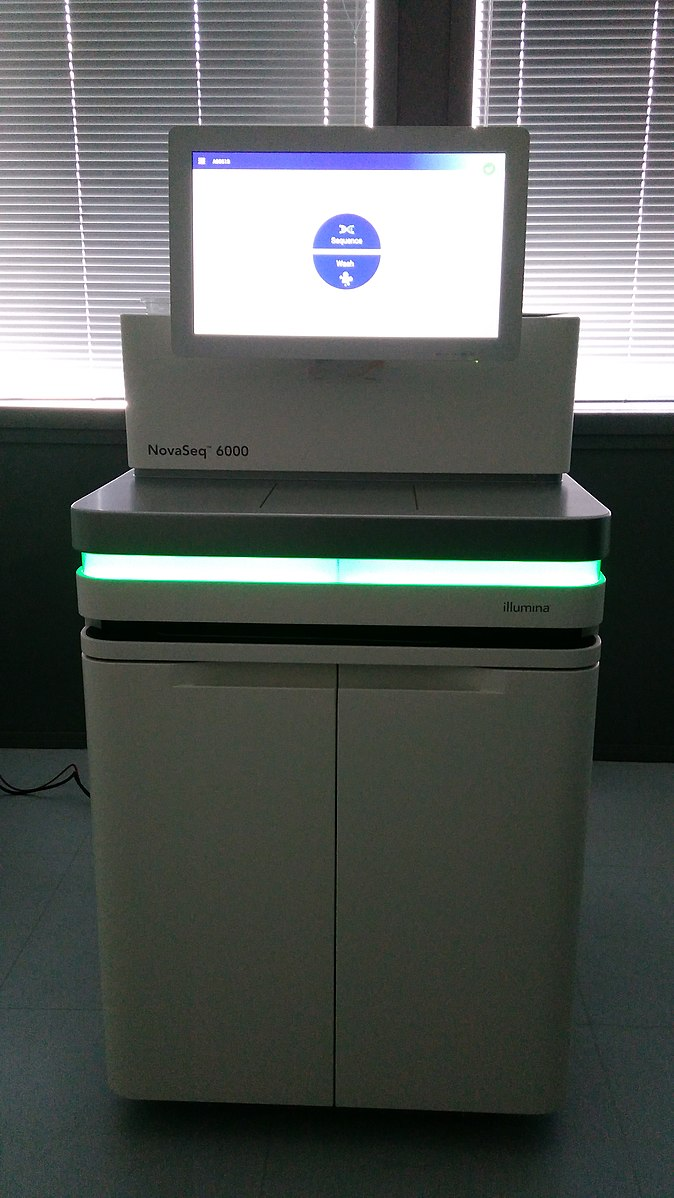
\includegraphics[height=5.2cm]{Kapitel/NGSTechnologien/Bilder/NGSNovaSeq.jpg}\\
					\vspace{0.3cm}\captionof{figure}{Das Großgerät des aktuellen Marktführers: Ein Illumina NovaSeq (ca. 10000M Reads je 300 bp, bis ca. 3 Tbp)\cite{NGSNovaSeq}}
                \end{center}
            \end{mdframed}
        \end{textblock}
    }
    \only<5->{
        \begin{textblock}{9.2}(5,3.4)
            \begin{mdframed}[backgroundcolor=white]
                \begin{center}
                    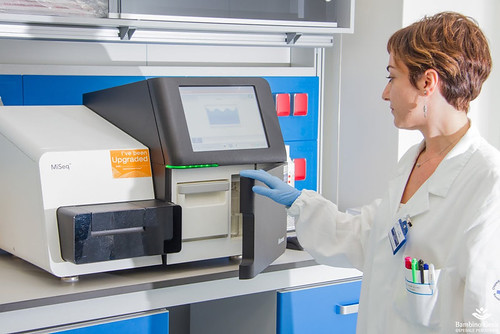
\includegraphics[height=5.2cm]{Kapitel/NGSTechnologien/Bilder/NGSMiSeq.jpg}\\
					\vspace{0.3cm}\captionof{figure}{Ein Kleingerät des aktuellen Marktführers: Ein Illumina MiSeq (ca. 25M Reads je 600 bp, bis ca. 15 Gbp)\cite{NGSMiSeq}}
                \end{center}
            \end{mdframed}
        \end{textblock}
    }
    \only<6->{
        \begin{textblock}{9.2}(6,3.5)
            \begin{mdframed}[backgroundcolor=white]
                \begin{center}
                    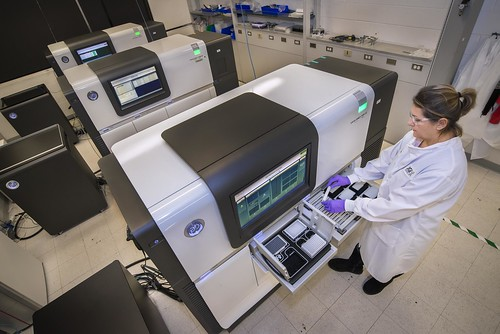
\includegraphics[height=5.2cm]{Kapitel/NGSTechnologien/Bilder/NGSPacBio.jpg}\\
					\vspace{0.3cm}\captionof{figure}{Großes 3rd Generation Sequencing-Gerät: Ein PacBio RSII (ca. 55K Reads je 15000 bp, bis ca. 900 Mbp)\cite{NGSPacBio}}
                \end{center}
            \end{mdframed}
        \end{textblock}
    }
    \only<7->{
        \begin{textblock}{9}(7,3.6)
            \begin{mdframed}[backgroundcolor=white]
                \begin{center}
                    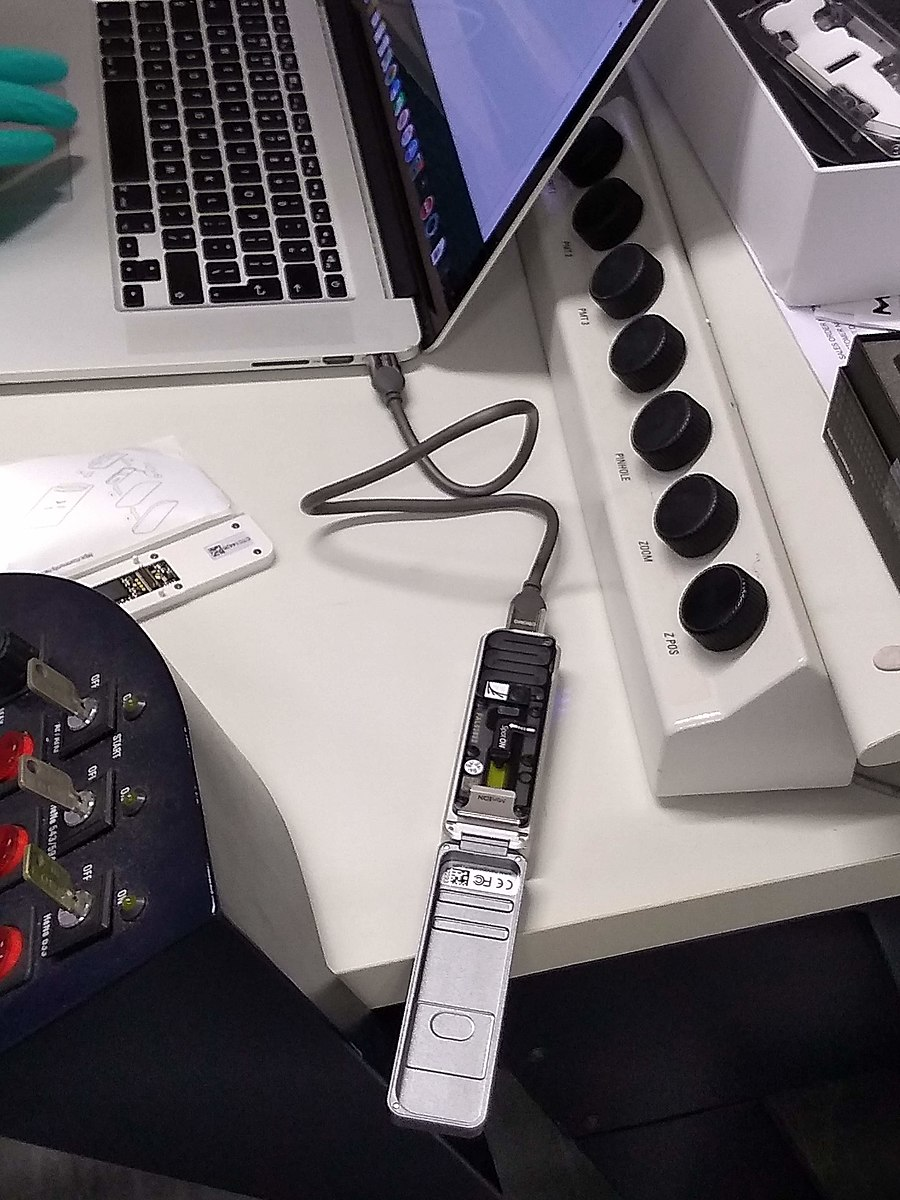
\includegraphics[height=5.2cm]{Kapitel/NGSTechnologien/Bilder/NGSMinION.jpg}\\
					\vspace{0.3cm}\captionof{figure}{Kleines 3rd Generation Sequencing-Gerät: Ein Oxford Nanopore MinION (bis zu 512 parallele Reads je bis ca. 2 Mbp, ca. 0.4 Mbp pro Stunde, bis ca. 50 Gbp)\cite{NGSMinION}}
                \end{center}
            \end{mdframed}
        \end{textblock}
    }
\end{frame}
